\documentclass{beamer}
%\usetheme{Antibes}
\usetheme{Dresden}
%\usetheme{Frankfurt}
%\usetheme{Copenhagen}
%\usetheme{Darmstadt}
%\usecolortheme{dolphin}
\usepackage{cancel}
\usepackage{tikz}
%%%%%%%%%%%%%%%%%%%%%%%%%%%%%%%%%%%%%%%%%%%%%%%%%%%%%%%%
\usepackage{multicol}

\newtheorem{proposition}[theorem]{Proposition}
\newtheorem{remark}[theorem]{Remark}
\newtheorem*{remark*}{Remark}
\newtheorem{conjecture}[theorem]{Conjecture}
\newtheorem{claim}[theorem]{Claim}
\newtheorem*{claim*}{Claim}
\usepackage{xcolor}
\usepackage{longtable}
\usepackage{hyperref}
\newtheorem{openproblem}[theorem]{Open Problem}


\setbeamertemplate{blocks}[rounded][shadow=true]

\setbeamertemplate{theorems}[ams style]
\begin{document}
	\title[]{\textcolor{black}{\textbf{Predict Rain in Australia.}}}
	
	\author[Yevgeniy Kostrov \hspace{1in} ekostrov@yahoo.com]
	{\textcolor{black}
	{\textbf{by Y.~Kostrov\inst}}}
	\date[April 14, 2019]

%
%	Title Page:
%	

%	{
%\usebackgroundtemplate{\includegraphics[height=\paperheight,width=\paperwidth]{london}}
%\frame{
%}
%}
	\begin{frame}	
			\maketitle
	\end{frame}
\begin{frame}{\contentsname}
	\begin{multicols}{2}
		\tableofcontents
	\end{multicols}
\end{frame}
%
%
%	
%
%
%}
\section{Overview}
\frame{
\frametitle{Overview }
\begin{center}
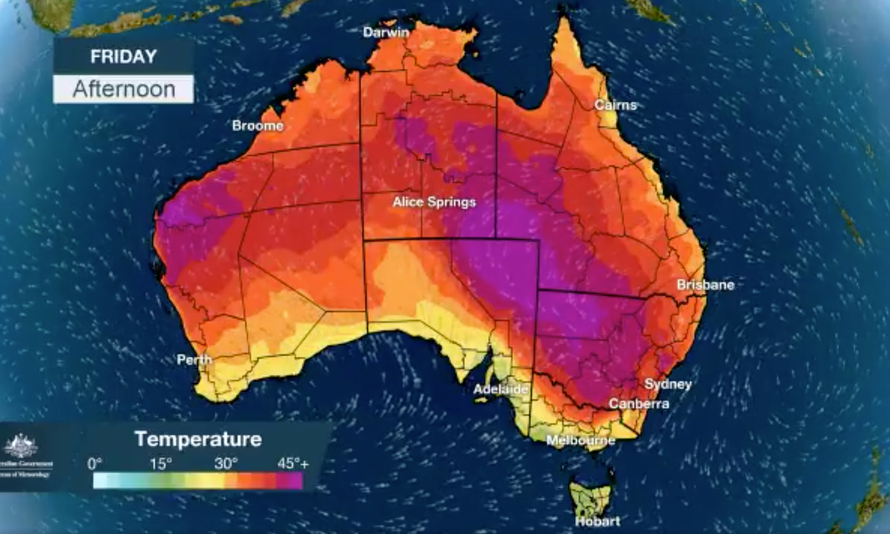
\includegraphics[width=2in]{../images/1786.png}\\
	The purpose of this project is to use weather data set from Kaggle to predict rainfall for the next day, based on the data about today's weather.
\end{center}
}
\section{Business Problem}
\frame{
\frametitle{Business Problem}
\begin{itemize}
	\item Predicting rainy weather for the next day is a very important task. 
	\item  Usually weather is predicted by using complicated deterministic models involving partial differential equations.
	\item  I will suggest a model that predicts weather by using Machine Learning.
\end{itemize}
}
\section{Data}
\frame{
\frametitle{Data Used in the Project}
\begin{itemize}
	\item This data set contains about 10 years of daily weather observations from many locations across Australia. 
	\vskip 0.2in
	\item RainTomorrow is the target variable to predict. It means -- did it rain the next day, Yes or No? This column is Yes if the rain for that day was 1mm or more.
\end{itemize}
}
\frame{
	\frametitle{Number of Rainy and Sunny days.}
	\begin{center}
		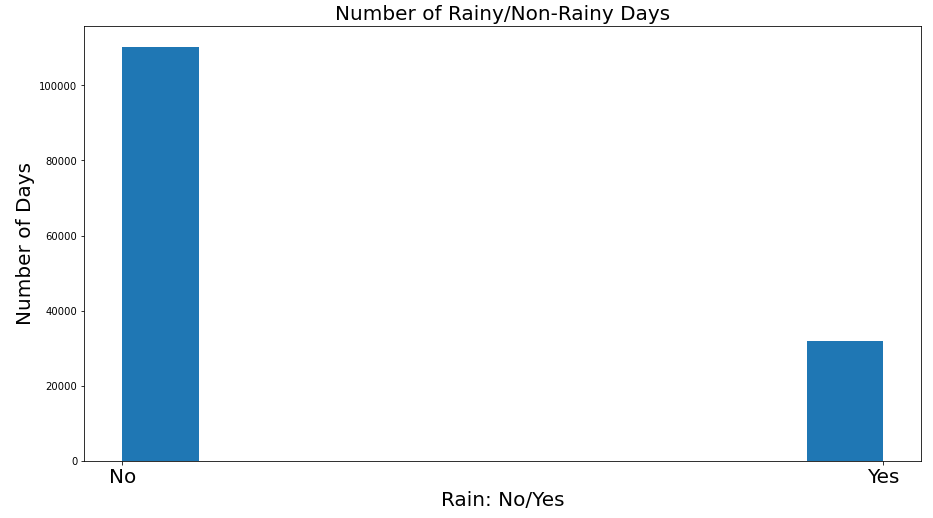
\includegraphics[width=4in]{../images/pic1.png}
	\end{center}
}
\frame{
	\frametitle{Rainy and Sunny days by Month.}
	\begin{center}
		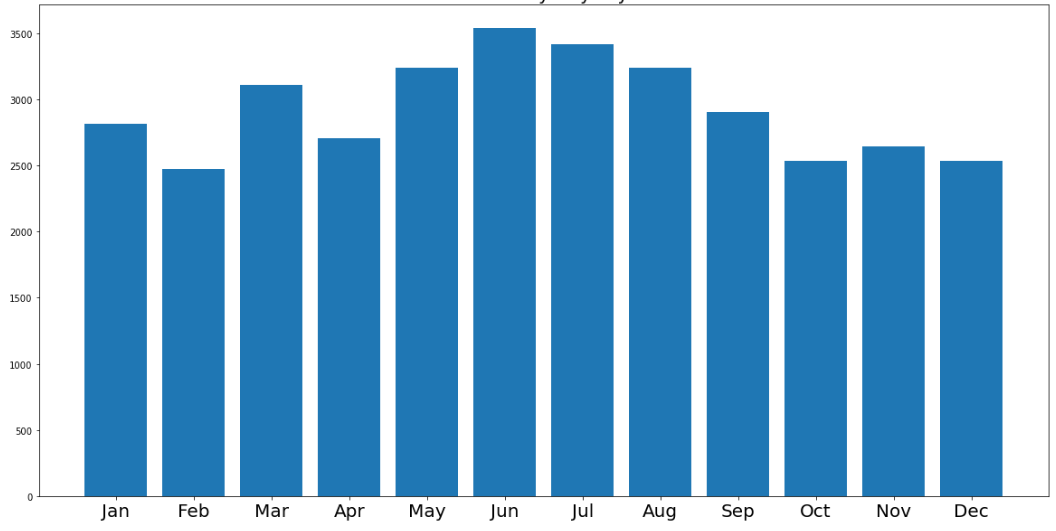
\includegraphics[width=4in]{../images/pic2.png}
	\end{center}
}
\section{Modeling}
\frame{
\frametitle{Modeling: Creating Baseline Models}
I have built the following two classifiers 
\vskip 0.1in
\begin{itemize}
	\item Logistic Regression Classifier
	\item Random Forest Classifier
	\item KNeighbors Classifier
	\item Support Vector Machines Classifier
	\item XG Boost Classifier
	\item Naive Bayes Classifier
\end{itemize}
}
\subsection{Metrics}
\frame{
\frametitle{Explanation of  Recall}
\begin{itemize}
	\item I used \textbf{recall} as a metric to select the base model and optimize by later on.
\item Recall is defined as:
\[\small \text{Recall} = \frac{\text{True Positive}}{\text{True Positive + False Negative}} = \frac{\text{True Positive}}{\text{Total Actual Positive}}\] 
\end{itemize}
}
\frame{
	\frametitle{Explanation of Recall}
\begin{itemize}
	\item Recall calculates how many of the Actual Positives our model captures by marking it as Positive (True Positive). 
	\item Thus Recall is a better model metric  when there is a high cost associated with False Negative.
	\item In our case False Negative is predicting "No Rain" when there is a "Rain Tomorrow".
\end{itemize}
}
\frame{
\frametitle{Explanation of Recall}
\begin{itemize}
	\item For instance, in rain prediction. 
	\item If it rains tomorrow (Actual Positive) is predicted as no rain tomorrow (Predicted Negative), then the person who relies on the prediction will be really upset since being unprepared for bad weather.
\end{itemize}
}
\frame{
\frametitle{Explanation of  Precision}
\begin{itemize}
	\item There is a secondary metric I will be watching, called "precision".
	\item Precision is defined as:
	\[\small \text{Precision} = \frac{\text{True Positive}}{\text{True Positive + False Positive}} = \frac{\text{True Positive}}{\text{Total Predicted Positive}}\]
	\normalsize 
\end{itemize}
}
\frame{
	\frametitle{Explanation of Precision}
	\begin{itemize}
		\item Precision describes how precise/accurate your model is out of those predicted positive, how many of them are actual positive.
		\vskip 0.2in
		\item Precision is a good measure when we worry about the costs of False Positive.
	\end{itemize}
}
\frame{
\frametitle{Explanation of Precision}
\begin{itemize}
	\item In our rain prediction, a false positive means "No Rain" tomorrow (actual negative) has been identified as "Rain" tomorrow.
	\item It is not that bad, since a person will carry an umbrella or rain coat for nothing.
\end{itemize}
}
\section{Models' Performance}
\frame{
\frametitle{How Well Baseline Models Performed}
\begin{itemize}
	\item 
\end{itemize}
}
\section{Conclusions}
\frame{
\frametitle{Conclusions}
\begin{itemize}
	\item
\end{itemize}
}
\frame{
\frametitle{Ways to Improve the Project}
\begin{itemize}
	\item I would like to optimize the code.
	\item Learn more about weather and related data.
\end{itemize}
}
\frame{
\begin{center}
	\LARGE
	THE END \\
	THANK YOU!
\end{center}
}
\end{document}
